\section{Modelos preditivos}

Dada a solução proposta, este trabalho estuda a viabilidade de dois modelos preditivos - previsão através de (1) geração de novas sequências e (2) indexação e identificação de sequências. Ambas baseiam-se em extrair informações a partir de entradas anteriores de áudio e apontar um \textit{output} sobre o que classificam ser o mais próximo do dado real futuro - no entanto, possuem diferenças sobre a forma como atingem esse objetivo.

\subsection{Geração de novas sequências}
\label{subsec:new_sequence_generator}

Gerar novas sequências baseando-se em entradas anteriores encaixa-se intuitivamente no conceito de ``previsão'', como descrito no algoritmo de \textit{client-side prediction}. Evidentemente, seu uso em uma adaptação para ambientes musicais foi explorado.

Em nossa adaptação do \textit{client-side prediction}, anteriormente à sessão entre os músicos, um modelo de aprendizagem de máquina é treinado utilizando áudios já conhecidos -  semelhantes, mas não iguais aos que serão produzidos pelo músico remoto. Este modelo receberá como entrada sequências de áudio de $t$ ms de duração e produzirá saídas de mesma duração, como descrito na \figref{fig:generative_model}.

\begin{figure}[htbp]
    \centering
    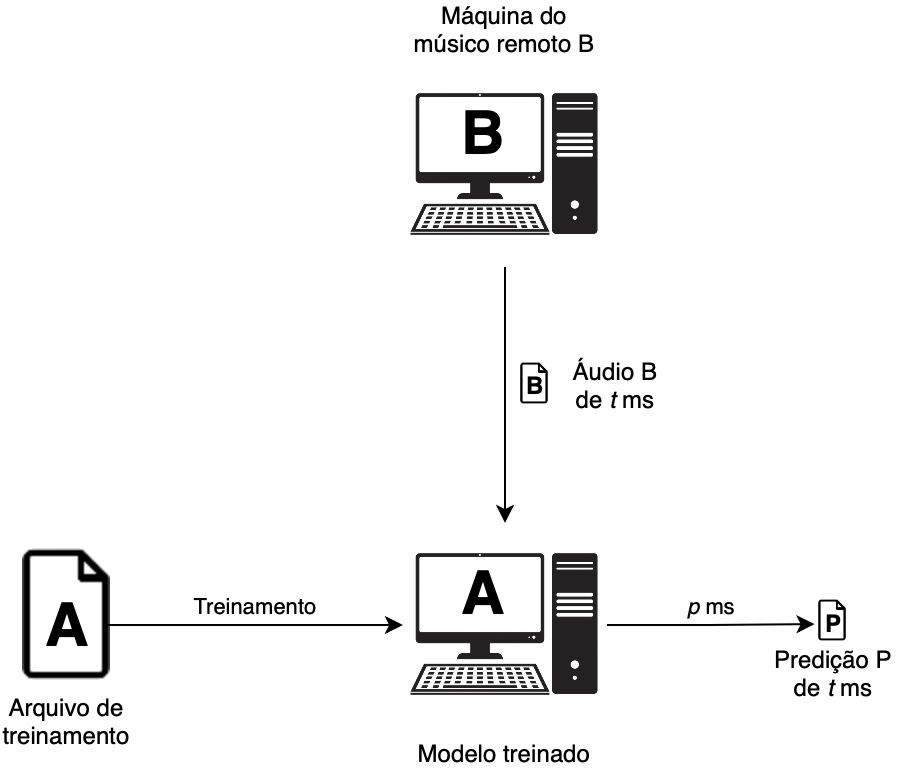
\includegraphics[width=0.75\textwidth]{images/prediction-model.png}
    \caption{Processo de geração de novas sequências através de modelos treinados.}
    \label{fig:generative_model}
\end{figure}

Uma das possibilidades para prever sequências musicais pode ser encontrado no campo de continuação de músicas baseados em um estilo. Dhariwal et. al propõem o \textit{Jukebox}, da \textit{OpenAI}, que usa redes neurais para aprender diferentes gêneros e produzir continuações para músicas \cite{jukebox}. Para o uso em previsões, poderíamos treinar modelos com a música a ser tocada e, para cada pequena sequência, gerar uma continuação. Entretanto, os autores deixam claro que uma das limitações de seu uso é o tempo de renderização - cerca de 8 horas para cada minuto de áudio gerado \cite{jukebox}. Como o tempo de geração das previsões é bastante sensível em nossa adaptação, essa abordagem foi descartada.

O campo da Aprendizagem de Máquina que visa gerar novas sequências baseando-se nas anteriores é a de Previsão de Séries Temporais (\textit{Time Series Forecasting}). Essa abordagem procura aplicar técnicas para prever continuações de conjunto de dados onde o tempo é uma de suas dimensões \cite{time_series_forecasting}. Podemos classificar, portanto, que previsões de sequências musicais é um subconjunto dos problemas desse campo e, dessa forma, adaptá-la para uso em nossa solução proposta.

Uma das abordagens utilizadas para resolver problemas do conjunto \textit{Time Series Forecasting} é a aplicação das redes neurais recorrentes LSTM (\textit{Long Short-Term Memory}) \cite{lstm}. Tais redes são capazes de aprender conexões de longo prazo. Dessa maneira, elas possuem um memorável poder de predição, funcionando bem em diversos problemas, sendo amplamente utilizadas atualmente.

A biblioteca \textit{Keras} \cite{keras}, escrita na linguagem de programação Python, implementa modelos de aprendizagem LSTM. Dessa forma, seu uso é bastante promissor para nossa adaptação musical de \textit{Client-Side Prediction}. Exploramos-o no primeiro ciclo de estudos, descrito no \chapref{chap:lstm}.

\subsection{Indexação e identificação de sequências anteriores}
\label{subsec:indexation_and_identification}

No primeiro ciclo de estudos, uma das possibilidades estudadas foi, ao invés de treinar um grande modelo, utilizar cada janela de previsão e treinar pequenos modelos. Para isso, no momento da previsão, precisaríamos de alguma forma de identificar qual modelo melhor se encaixa na sequência de entrada. Com isso, pesquisamos métodos para realizar a identificação das sequências de um banco de dados e, com isso, surgiu a ideia de, ao invés de gerar novas sequências, apenas entregar a que veio após a identificada. 

Para previsão de sequências, a geração de novos valores não é um requisito. Se possuirmos um conjunto de dados, reunindo diferentes sequências e informações sobre quais vieram após tais sequências, poderíamos apenas reproduzi-las. Dessa forma, sugerimos um modelo preditivo que, ao invés de fornecer sequências de áudio inéditas, identifica sequências similares e reproduz a que veio em seguida, como ilustrado na \figref{fig:indexative_model}.

\begin{figure}[htbp]
    \centering
    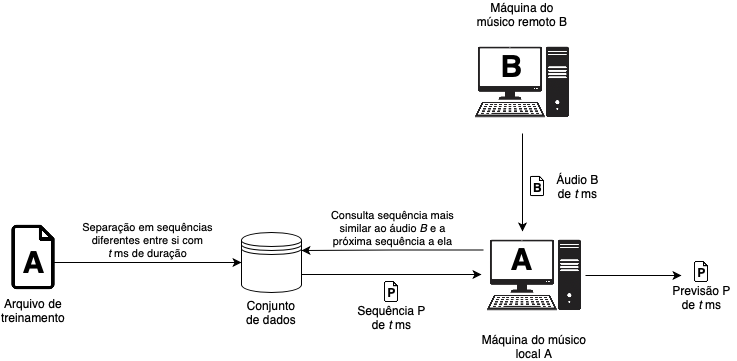
\includegraphics[width=1\textwidth]{images/index-model.png}
    \caption{Processo de identificação de sequência semelhante à entrada $B$ e entrega da previsão $P$, baseada na que veio após a sequência identificada.}
    \label{fig:indexative_model}
\end{figure}

Além do conjunto de regras apresentados na \secref{sec:data_gathering}, o conjunto de dados de referência que será consultado nesse modelo possui as seguintes regras:

\begin{enumerate}
    \item Todos os arquivos necessitam representar diferentes sessões da música entre si;
    \item Todos os arquivos necessitam possuir duração maior ou igual à $t$ ms, onde $t$ é a duração do arquivo utilizado para consulta de similaridade;
    \item Todos os arquivos requerem que exista um, e apenas um, arquivo que represente a sequência tocada após ele mesmo.
\end{enumerate}

A Regra 1 garante que, ao realizar uma \textit{query} de similaridade entre a sequência de entrada e as armazenadas, haverá no máximo uma correspondência. Tal requisito é importante, pois, se houver mais de uma, haverá mais de uma previsão, causando ambiguidade. A Regra 2 garante que as previsões entregues possuirão pelo menos a mesma duração que as sequências de entrada. Caso sejam menores, a diferença entre as durações causará um atraso de entrega, causando o problema descrito na \subsecref{subsec:time_metric}. Finalmente, a Regra 3 garante que todos os arquivos necessitam possuir outro que represente o que foi tocado após ele, que será de fato entregue como previsão, evitando ambiguidades.

Portanto, tal modelo requer duas técnicas: (1) uma para indexar as sequências de música, respeitando as regras descritas e (2) uma para identificar similaridade entre a sequência de entrada (transmitidas pelo músico remoto) e as sequências armazenadas.

Neste trabalho, realizamos a primeira técnica manualmente. O processo é demonstrado no \chapref{chap:dtw}.

Para a segunda técnica, estudamos alguns que métodos podem ser utilizados para identificação de sequências. A biblioteca Librosa \cite{librosa}, também escrita em Python, implementa algumas ferramentas que podem auxiliar em tal tarefa, como o cálculo da centroide espectral \cite{centroid} de sequências de áudio, que encontra uma média central entre as frequências presentes em cada janela de tempo da sequência de entrada. Para identificação, poderíamos pré-calcular as centroides de cada sequência no conjunto de dados e comparar com a sequência transmitida pelo músico remoto. Entretanto, apenas a informação das frequências principais não é suficiente para identificar semelhança, uma vez que tal informação não varia tanto para cada janela, principalmente para aquelas que reproduzem o mesmo acorde ou nota.

A mesma biblioteca implementa o algoritmo DTW (\textit{Dynamic Time Warping}) \cite{dtw}, um algoritmo utilizado para comparar e alinhar duas séries temporais. Em nossa adaptação de \textit{client-side prediction}, podemos aplicar DTW nas sequências transmitidas contra o banco de dados. Caso haja uma janela semelhante, o algoritmo a entregará como \textit{output} os \textit{timestamps} representando o início e fim da identificação.

Dessa forma, o \chapref{chap:dtw} também demonstra como utilizamos o DTW em nossas experimentações, além de sua taxa de sucesso na identificação de janelas semelhantes. Caso essa taxa seja alta o suficiente e a indexação das previsões seja acurada, será possível reproduzir um áudio bastante similar ao transmitido pelo músico remoto.

\subsection{Comparações entre os modelos}

Apesar de ambos os modelos basearem-se em sequências anteriores para gerar ou apontar previsões musicais, as duas abordagens diferem na forma que funcionam. As diferenças implicam em alguns pontos que uma abordagem pode realizar melhor que a outra, assim como o inverso pode ocorrer, descritos na \tabref{tab:models_comparission}.

\begin{table}[ht!]
    \centering
    \begin{tabular}{|c|c|c|c|c|}
        \cline{2-5}
        
        \multicolumn{1}{c|}{} & \rotatebox[origin=c]{90}{\makecell{Flexível a \\ novas entradas}} &
        \rotatebox[origin=c]{90}{\makecell{Requer pouca \\ informação}} & \rotatebox[origin=c]{90}{\makecell{Predição de \\ alta resolução}} &
        \rotatebox[origin=c]{90}{\makecell{Rápido \\ processamento}} \\
        
        \hline
        
        Modelo gerador & X & X & & \\ 
        \hline
        
        Modelo indexador & & & X & X \\ 
        \hline
    \end{tabular}
    \caption{Matriz morfológica comparando os dois modelos propostos para adaptação do \textit{client-side prediction} para música.}
    \label{tab:models_comparission}
\end{table}

Por entregar sequências inéditas, o modelo preditivo gerador de novas sequências, descrito na \subsecref{subsec:new_sequence_generator}, é mais flexível que o modelo indexador, descrito na \subsecref{subsec:indexation_and_identification}. Afinal, entradas nunca vistas anteriormente sempre terão previsões geradas, mesmo que não sejam precisas com a realidade. Se aplicarmos sequências não vistas no modelo indexador, nenhuma janela será identificada e, portanto, nenhuma previsão poderá ser realizada acuradamente.

Além disso, para identificar uma janela precisamente, o modelo indexador requer mais informações que o modelo gerador, aumentando, portanto, o tempo da janela de previsão. Quanto maior a janela prevista, mais suposições terão que ser feitas sobre a previsão e, portanto, menor a probabilidade de replicar, de forma similar, a sequência de entrada. 

Por outro lado, pela natureza complexa da representação de áudio, gerar uma sequência de alta qualidade de definição sonora, ainda que semelhante à sequência real do músico remoto, é um grande desafio para o modelo gerador. Por entregar sequências já armazenadas em alta qualidade, o modelo indexador sempre entregará sequências limpas ao ouvido humano, evitando desconfortos dos músicos.

Ademais, a utilização de LSTM, devido à complexidade das redes neurais, pode requerer grandes tempos de processamento \cite{lstm_slow} para gerar as previsões. A busca com DTW, apesar de ser um algoritmo de complexidade $O(N^2)$, pode ser otimizado para grandes bases de dados \cite{dtw_complexity}. Como o tempo de previsão é sensível em nossa adaptação do \textit{client-side prediction} para música, é essencial que o modelo preditivo seja eficiente.
